
O Banco de Dados do AnaclaraBot tem 3 coleções, são elas:
\begin{enumerate}

\item \textbf{User:} Contém os dados dos usuários que se cadastraram, e as referências para as conversas (\emph{Conversations}), as quais ele participou.

\item \textbf{Conversation:} Contém os meta-dados das conversas, referências para as interações (\emph{Interactions}) e um ou vários \textit{quizzes} que o usuário responde ao final do chat.

\item \textbf{Interaction:} Contém a pergunta do usuário, resposta do bot, os \textit{intents} e as \textit{entities}. Tanto a pergunta do usuário quanto a resposta do bot podem ser em formato de texto, áudio ou imagem.

\end{enumerate}


\par O modelo do Banco de Dados está descrito na Figura \ref{fig:diagram}.
\begin{figure}[!ht]
  \centering
      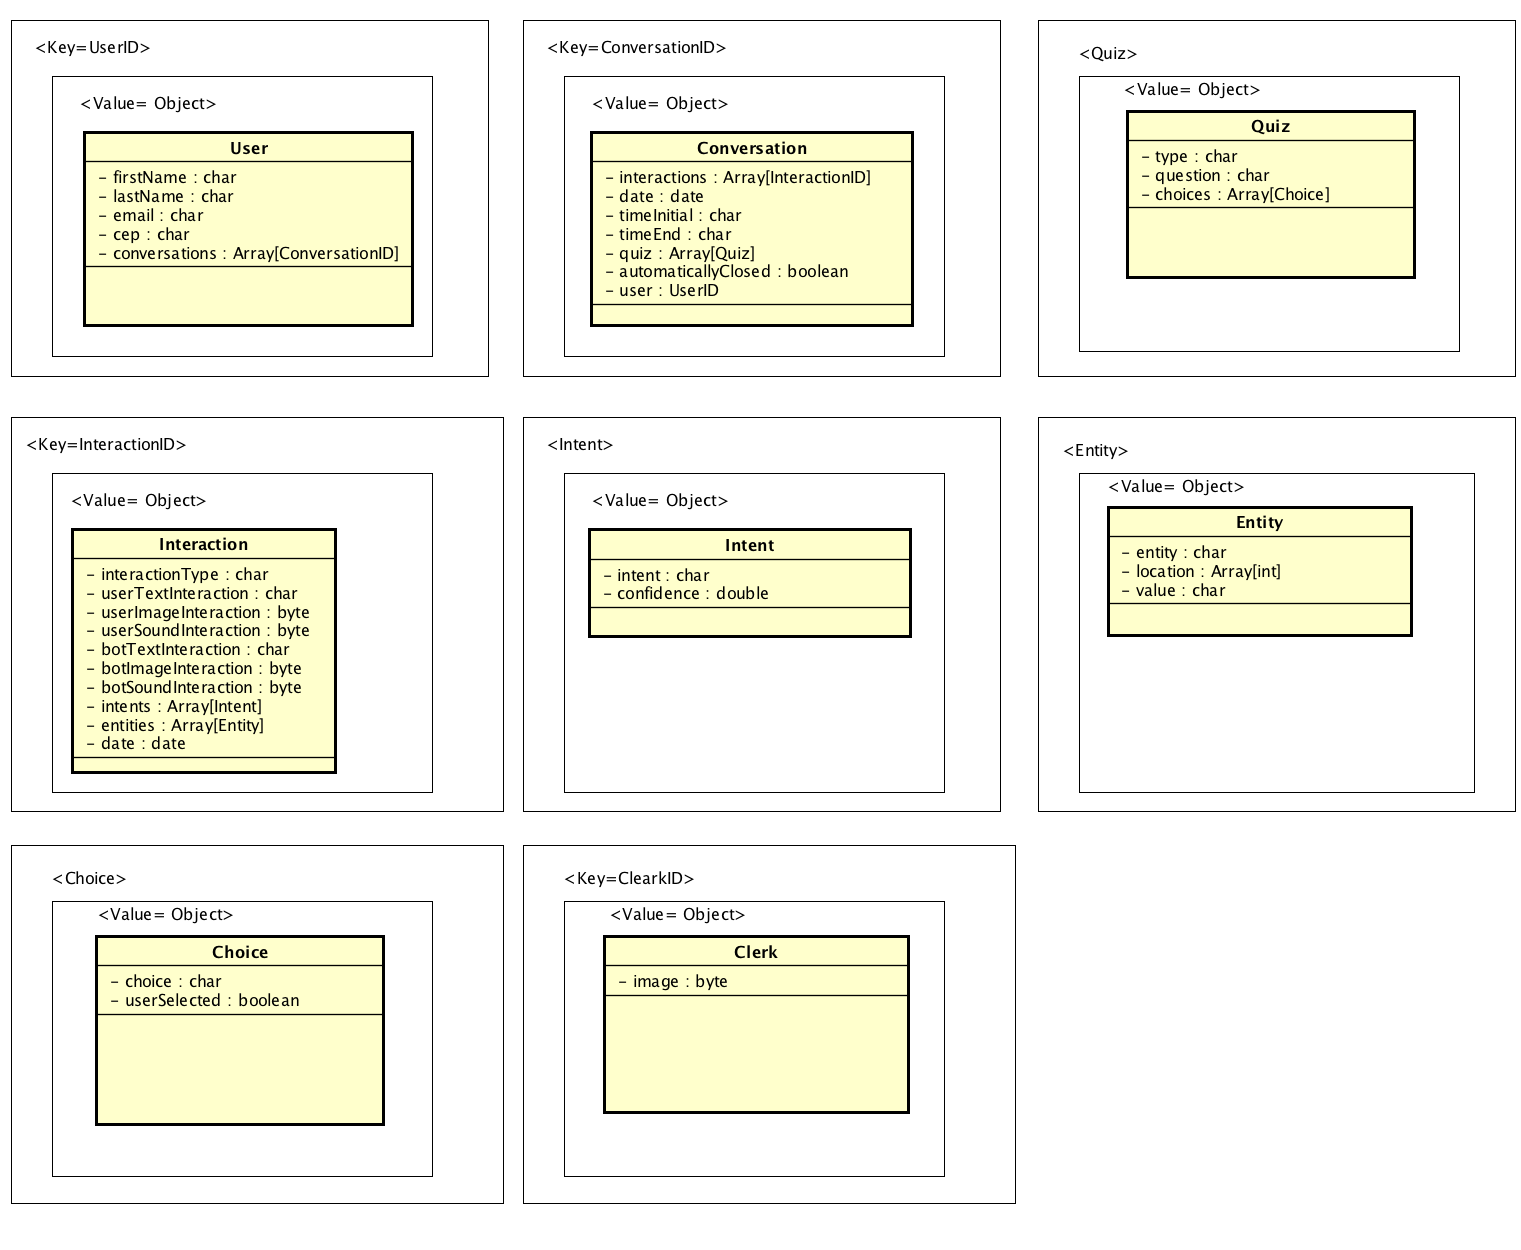
\includegraphics[width=0.9\textwidth]{diagram}
  \caption{Modelo do Banco de Dados}
  \label{fig:diagram}
\end{figure}
